\documentclass[11pt,twocolumn]{article}

\usepackage[margin=1in]{geometry}
\usepackage{amsmath,amssymb}
\usepackage{graphicx}
\usepackage[T1]{fontenc}
\usepackage[utf8]{inputenc}
\usepackage{natbib}
\usepackage[colorlinks=true,citecolor=blue,linkcolor=black,urlcolor=blue]{hyperref}

\title{An implementation of Kass snakes in Python}
\author{Hunter}
\date{}

\begin{document}
\maketitle

\section{Introduction}

Active contour models are commonly used to locate object boundaries in images. Kass, Witkin, and Terzopoulos introduced snakes as energy-minimizing splines guided by internal smoothness, image features, and external constraints \cite{kass1988snakes}. Because the published model is continuous, turning it into a discrete contour requires a stiffness matrix, a force sampling method, and a stable time-step scheme.

A snake is an energy-minimizing spline with internal, image, and constraint terms \cite{kass1988snakes}. Instead of needing an edge map of the image, it uses tension and bending to keep the contour smooth, and line, edge, and termination functionals to pull toward image features. Springs and volcanoes act during the solve.

The discrete snake is a closed ring of vertices. Tension at a vertex depends on its two immediate neighbors. Bending also depends on the vertices two steps away, so each vertex is tied to five points in all. Those couplings are stored as a pentadiagonal stiffness matrix: five nonzero diagonals, wrapping around at the ends because the contour is a loop. If the code just added the current smoothness and image forces and stepped forward, the bending term would throw the vertices around unless the time step were tiny. Implicit Euler avoids that by solving a linear system for the next positions, so the new contour already balances smoothness against the image force \cite{kass1988snakes}. That is the update used here.

In this assignment, the implementation is Python with NumPy and OpenCV, using closed snakes and bilinear sampling of the image force at each vertex. This implementation has two stages. First, the user draws one or more closed snakes as a circle or a polyline, and the contours evolve under image energy. Second, during the live solve the user can pull vertices with springs, push them with volcanoes, change the Gaussian scale of the image energy, or start auto-finish. Auto-finish is an unattended multi-scale run that stops when every snake has settled.

This report walks through that Python implementation on one synthetic image. Each energy is written as code, then shown on the same contour.

\section{Methods and results}

The vertices from the introduction are the beads of the snake. This section writes each 1988 energy as code and shows what it does to those beads on one image. The image is synthetic: a white disk joined to a white square, and a short black stroke set off to the side. The disk is a round edge. The square adds sharp corners. The stroke is a line apart from that blob.

\subsection{Initialization}

Kass gives the energies of a snake that already exists. The user supplies the first contour. A circle is a center click and a rim click. A polyline is a run of clicks that the program closes. Either outline is then filled in to a working loop of beads. With the default density of $0.5$, the spacing is about one bead every four pixels of perimeter, and a circle keeps at least eight beads. Figure~\ref{fig:init} shows both modes. Yellow dots are the clicks. The red loop is the beads. Later figures use the circle.

The live program then runs with a fixed set of constants. Kass states the energies and the implicit step; these are the values chosen for this implementation. Each one is used in the subsection named with it.
\begin{itemize}
  \item $\alpha=0.08$, $\beta=0.40$: tension and bending (internal energy).
  \item $\gamma=0.10$, $\kappa=1$: stay near the current contour, and weight the image force (iteration).
  \item $w_{\mathrm{line}}=0$, $w_{\mathrm{edge}}=1$, $w_{\mathrm{term}}=0$, $\sigma=3$: which image term is on, and the blur width (image energy).
  \item Step cap of $1$~px on each axis; spring stiffness $0.08$; volcano strength $900$, crater $20$~px (iteration and external energy).
\end{itemize}

\begin{figure}[t]
  \centering
  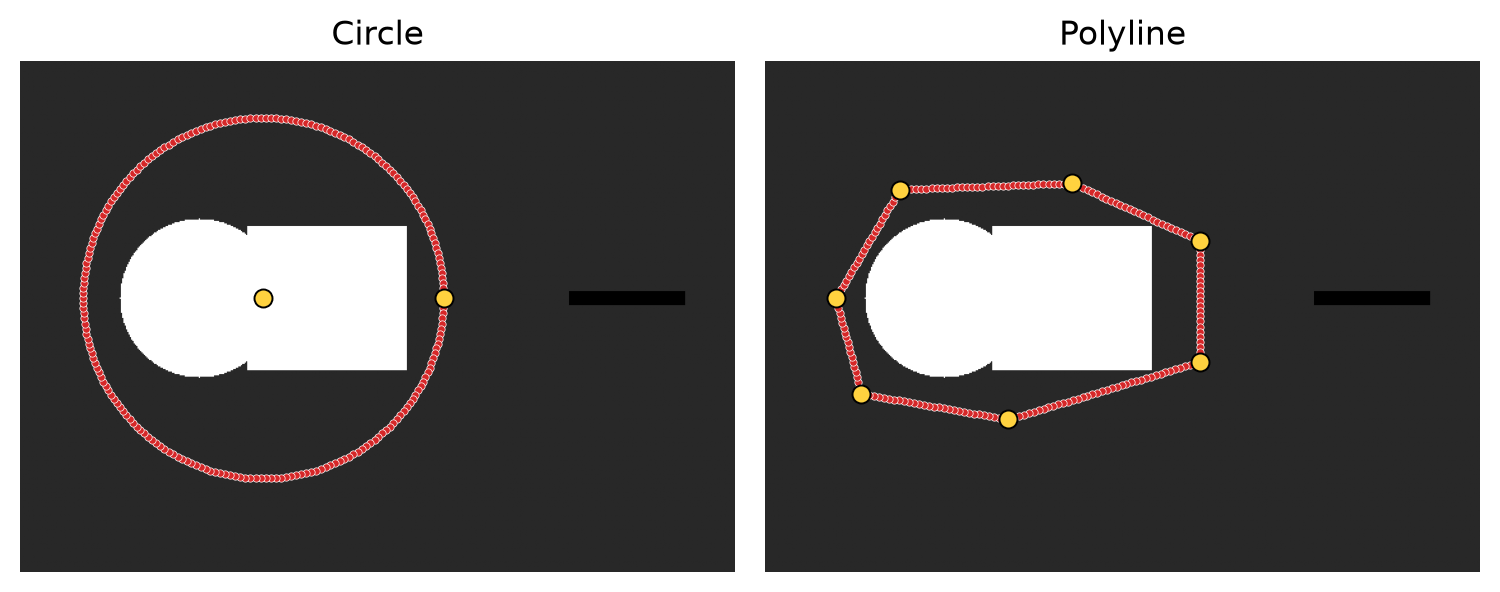
\includegraphics[width=\linewidth]{images/init.png}
  \caption{Initialization. Left: a center click and a rim click become a circle of beads. Right: polyline clicks are closed and filled in. Yellow dots are the clicks. Red is the bead loop.}
  \label{fig:init}
\end{figure}

\subsection{Internal energy}

Internal energy is tension plus bending \cite{kass1988snakes}. Tension, weighted by $\alpha$, pulls neighboring beads back together when they spread apart. Bending, weighted by $\beta$, pulls a kink back toward a smoother arc. This run uses $\alpha=0.08$ and $\beta=0.40$.

The coupling is two finite-difference stencils on the bead index. Spacing is $h=1$, one step in index. The ends wrap, because the contour is a loop. At bead $i$,
\begin{align}
  (D_2 v)_i &= v_{i-1} - 2v_i + v_{i+1}, \\
  (D_4 v)_i &= v_{i-2} - 4v_{i-1} + 6v_i - 4v_{i+1} + v_{i+2}.
\end{align}
$D_2$ is tension. $D_4$ is bending.

In code each stencil is the identity matrix, rolled left and right, so the wrap is built in and every bead is included in one product. One $\alpha$ and one $\beta$ are used for the whole snake, so
\begin{equation}
  A = -\alpha D_2 + \beta D_4.
\end{equation}
$A$ is built once from the number of beads, $\alpha$, and $\beta$. It does not depend on where the beads sit. Figure~\ref{fig:stiffness} is that matrix for a 16-bead loop. Applying $A$ to the current positions is the internal pull on every bead at once (Figure~\ref{fig:internal}).

\begin{figure}[t]
  \centering
  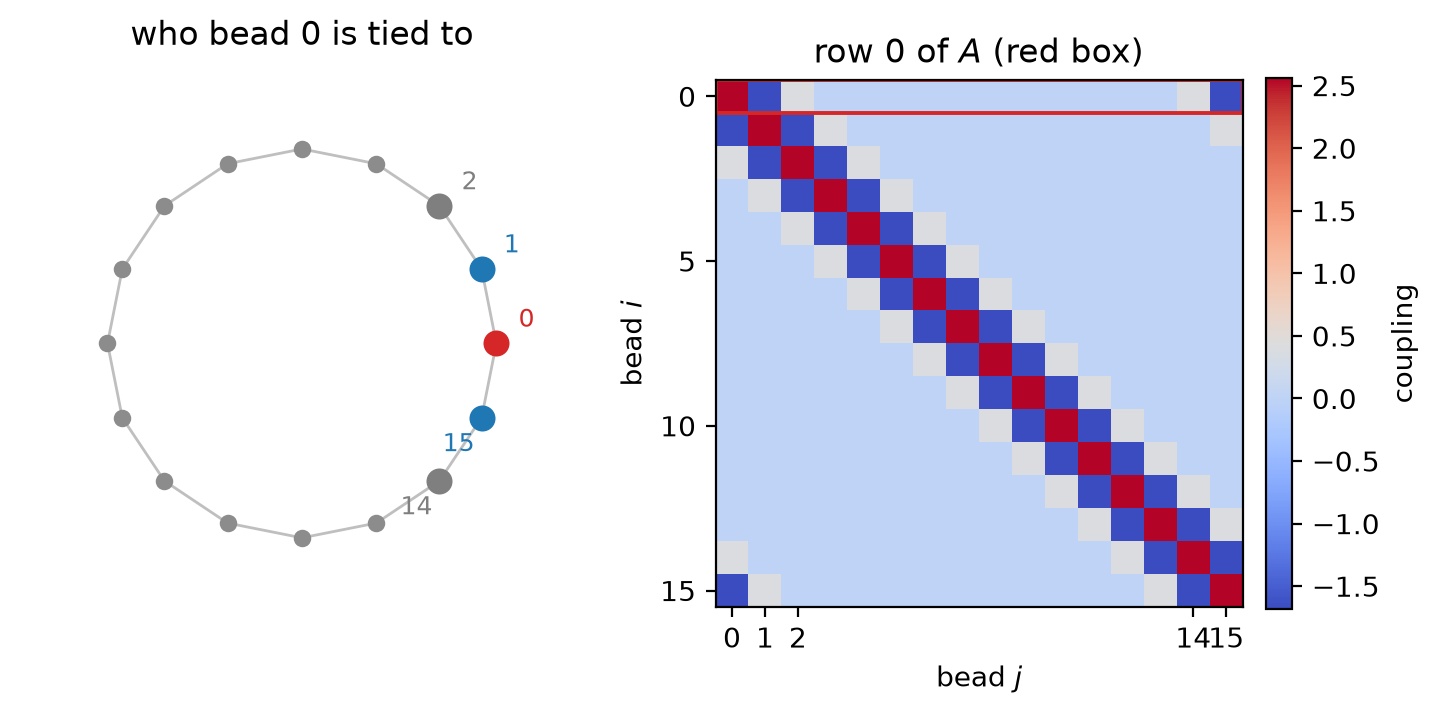
\includegraphics[width=0.95\linewidth]{images/stiffness_matrix.png}
  \caption{A 16-bead loop, and the weights in $A$. Pale blue is zero. The ring shows who bead 0 is tied to; the red box is row 0.}
  \label{fig:stiffness}
\end{figure}

\begin{figure}[t]
  \centering
  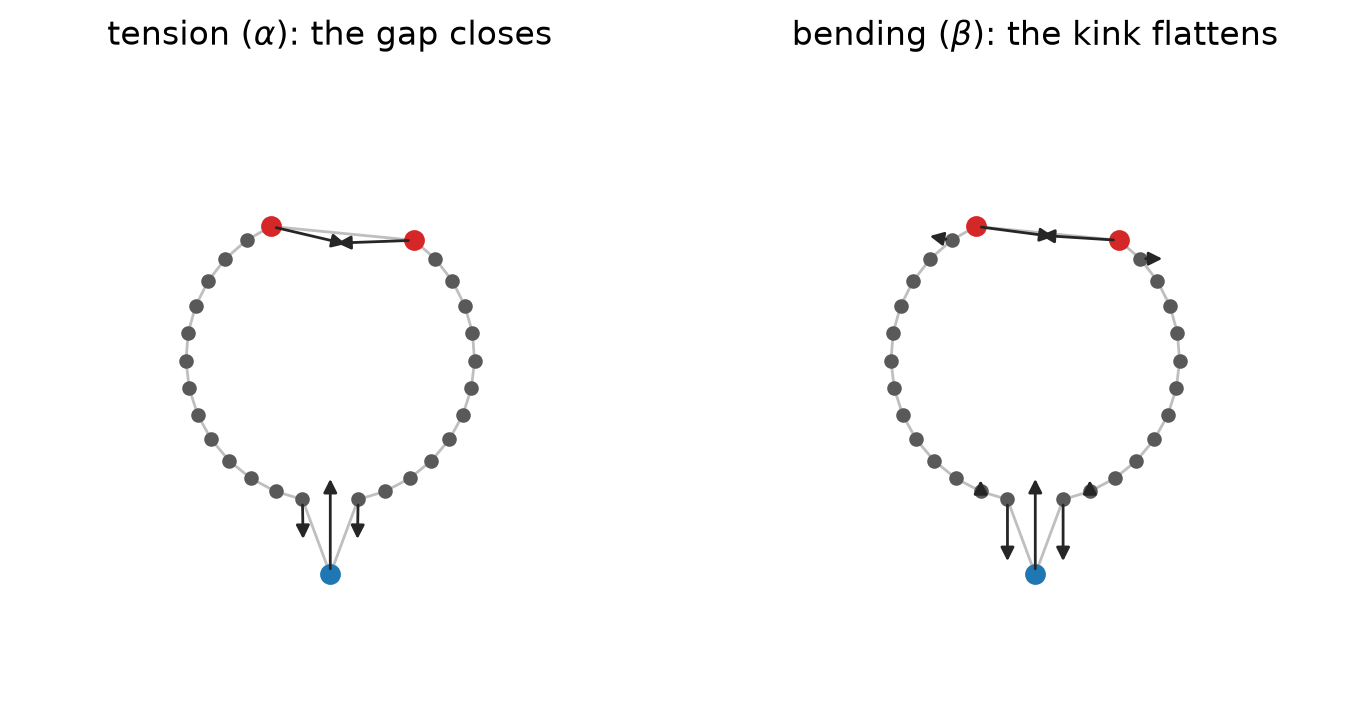
\includegraphics[width=0.95\linewidth]{images/internal_forces.png}
  \caption{Internal pull on a loop with a gap (red) and a kink (blue). Left: tension points across the gap. Right: bending points the kink back toward the loop. Arrow length is scaled separately in each panel.}
  \label{fig:internal}
\end{figure}

\subsection{Image energy}
\label{sec:image-energy}

Image energy is the weighted sum \cite{kass1988snakes}
\begin{equation}
  E_{\mathrm{image}}
    = w_{\mathrm{line}} E_{\mathrm{line}}
    + w_{\mathrm{edge}} E_{\mathrm{edge}}
    + w_{\mathrm{term}} E_{\mathrm{term}}.
\end{equation}
In code this sum is a pixel field. Beads sample it later.

The field starts with the image scaled to $[0,1]$ and blurred with \texttt{cv2.GaussianBlur} at width $\sigma$. This run uses $\sigma=3$. First and second derivatives of that blur are OpenCV Sobel filters \cite{bradski2000opencv}.

Line energy is the blurred intensity,
\begin{equation}
  E_{\mathrm{line}} = I.
\end{equation}
With a positive $w_{\mathrm{line}}$, dark pixels are the low-energy place, and the beads move toward dark lines. With a negative $w_{\mathrm{line}}$, bright pixels are the low-energy place, and the beads move toward light lines.

Edge energy is
\begin{equation}
  E_{\mathrm{edge}} = -(I_x^2 + I_y^2) = -|\nabla I|^2.
\end{equation}
The code squares and adds the first-order Sobel outputs, then negates. A strong gradient is a well, so a bead that reaches an edge stays there.

Termination energy is the curvature of the level lines of the blurred image \cite{kass1988snakes}. It is large at corners and at the ends of a stroke, and smaller along a gentle curve. The code takes $I_{xx}$, $I_{yy}$, and $I_{xy}$ from second-order Sobel:
\begin{equation}
  E_{\mathrm{term}}
    = \frac{I_{yy}I_x^2 - 2I_{xy}I_x I_y + I_{xx}I_y^2}
           {(I_x^2 + I_y^2 + \varepsilon)^{3/2}},
\end{equation}
with $\varepsilon = 10^{-8}$ so a flat region does not divide by zero.

The three arrays are combined with the weights, then divided by their maximum absolute value, so the step size does not depend on raw Sobel units. This run, and the live defaults, use $w_{\mathrm{line}}=0$, $w_{\mathrm{edge}}=1$, $w_{\mathrm{term}}=0$. Line and termination are still computed, so those weights can be turned on. Figure~\ref{fig:image-energy} shows each term on its own, before that mix.

Image force is $\nabla E_{\mathrm{image}}$. The code takes that gradient with \texttt{np.gradient} on the combined field.

A bead sits between pixel centers. The force at that bead is a bilinear blend of the four surrounding force pixels, so the value changes smoothly as the bead moves from one pixel to the next. With $d_x$ and $d_y$ the fractional offsets, and $F_{00}$, $F_{10}$, $F_{01}$, $F_{11}$ the samples at those four pixels,
\begin{equation}
  \begin{aligned}
  f &= (1-d_y)\big[(1-d_x)F_{00} + d_x F_{10}\big] \\
    &\quad + d_y\big[(1-d_x)F_{01} + d_x F_{11}\big].
  \end{aligned}
\end{equation}

\begin{figure*}[t]
  \centering
  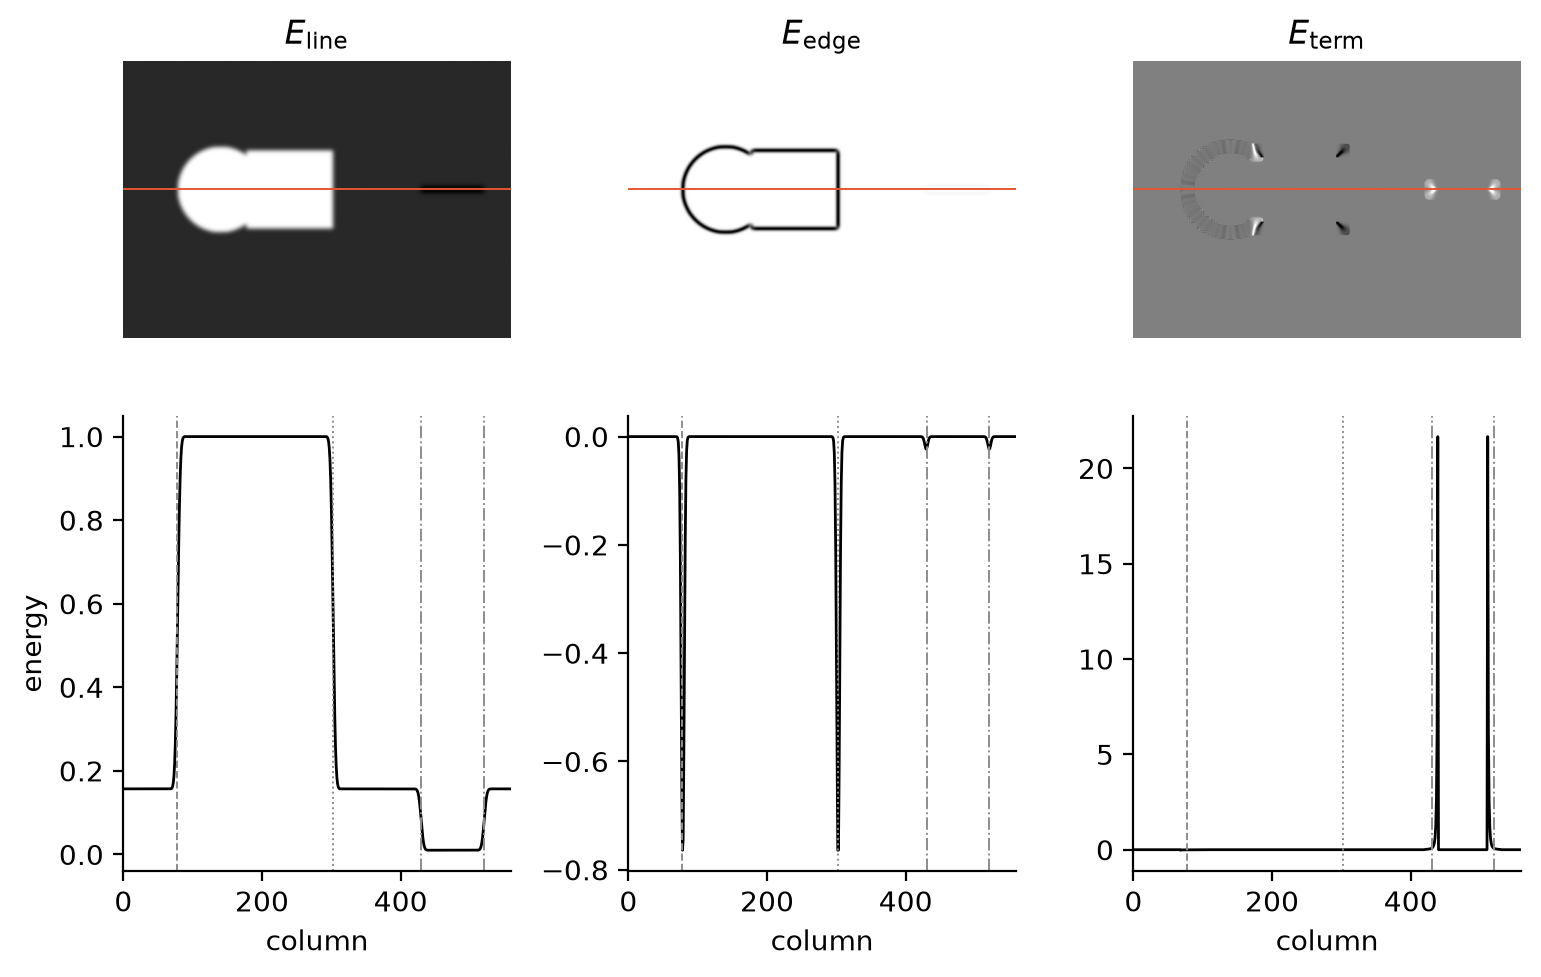
\includegraphics[width=\textwidth]{images/image_energy.png}
  \caption{Line, edge, and termination energy, each before the weighted mix. Darker is lower. The orange line is the plotted row. Dashed marks the disk's outer edge, dotted the square's outer edge, and dash-dot the ends of the stroke. Along that row, line energy is a high plateau on the white shape and a dip on the black stroke. Edge energy is a well at each boundary the row crosses. Termination stays near zero across the disk and the square, and spikes at the two ends of the stroke. The square's corners lie off this row. In the termination image those corners are dark, the stroke ends are bright, and the disk's boundary is only a faint curve. Termination is scaled so the corners and the stroke ends read; larger values saturate.}
  \label{fig:image-energy}
\end{figure*}

\subsection{External energy}

Constraint energy is how a user pushes on the snake while it moves \cite{kass1988snakes}. After the beads are drawn, this implementation uses a Snake Pit: springs and volcanoes placed with the mouse.

The sampled image force is scaled by $\kappa$. Springs and volcanoes are added after that scale, and the implicit step uses the sum.

A spring between bead $v_i$ and an anchor $a$ has
\begin{equation}
  E_{\mathrm{spring}} = \tfrac{1}{2} k \lvert v_i - a \rvert^2,
  \qquad
  \nabla E_{\mathrm{spring}} = k(v_i - a),
\end{equation}
with $k=0.08$. Left-dragging a bead attaches a spring. Releasing on empty space pins the anchor, and that bead is pulled toward the pin. Releasing on another bead, on any snake, ties the two together.

A volcano at $p$ is a $1/r$ repulsion, with strength $c=900$, cut off inside a crater of radius $r_0=20$~px \cite{kass1988snakes}:
\begin{equation}
  E_{\mathrm{volcano}} = \frac{c}{\lvert v-p \rvert}
  \quad (r > r_0),
  \qquad
  \nabla E_{\mathrm{volcano}} = -c\,\frac{v-p}{\lvert v-p \rvert^3}.
\end{equation}
A click places a volcano that stays put. Right-dragging, or the mouse-volcano toggle, puts $p$ at the cursor. Beads outside the crater are pushed away from $p$. Beads inside feel nothing.

Figure~\ref{fig:constraints} shows both on the running example. Figure~\ref{fig:fixing-corners} uses a spring on one corner of the square.

\begin{figure}[t]
  \centering
  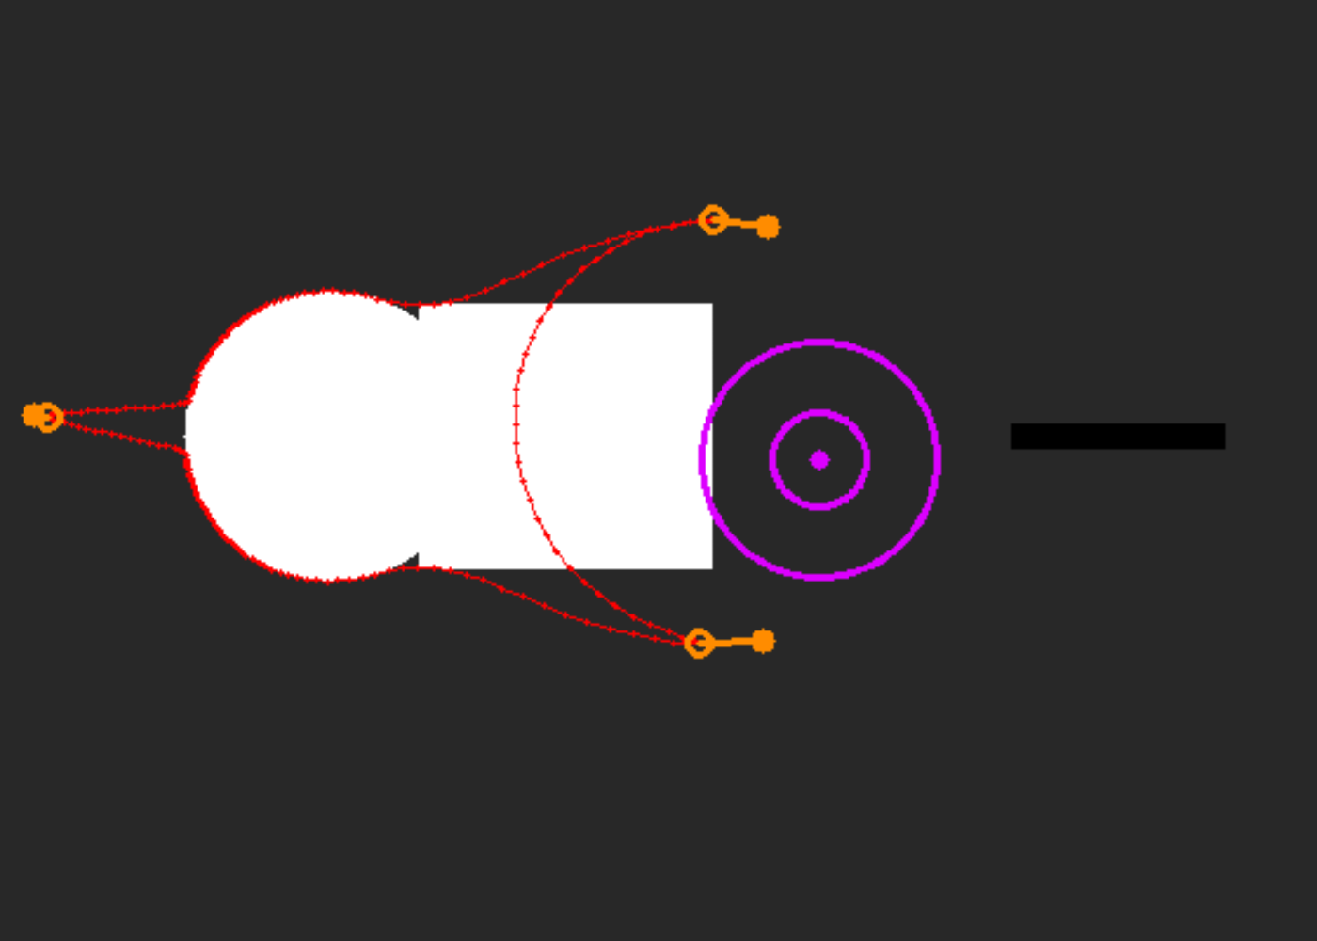
\includegraphics[width=\linewidth]{images/constraints2.png}
  \caption{Springs pull beads outward on the left. The volcano on the right pushes beads away, so the contour bends in on that side.}
  \label{fig:constraints}
\end{figure}

\begin{figure}[t]
  \centering
  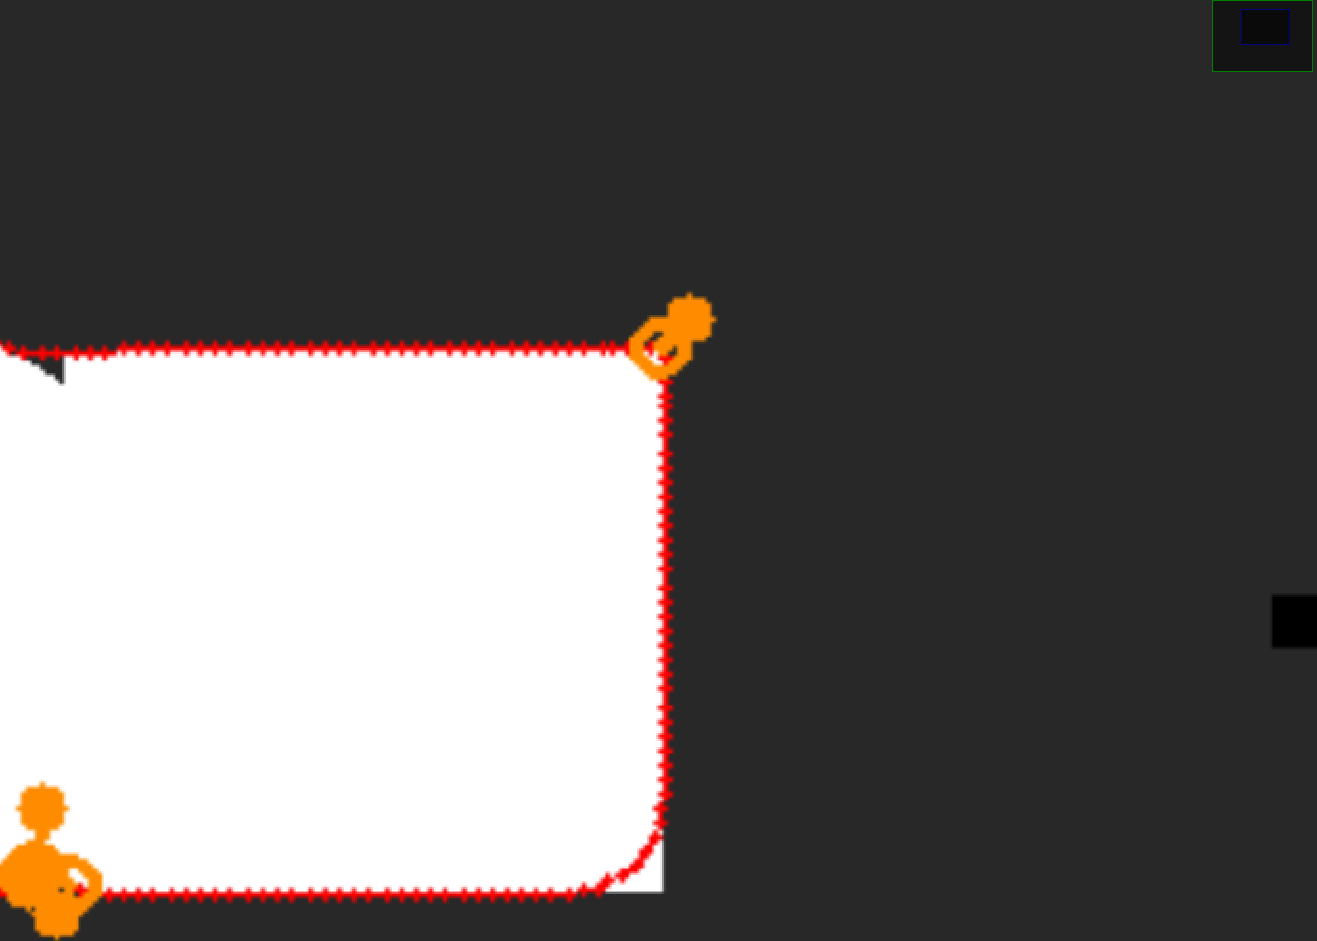
\includegraphics[width=\linewidth]{images/fixing_corners.png}
  \caption{A spring fixes one corner of the square. The orange pin on the top-right corner pulls that bead out, so the contour turns a sharp corner there. The pin on the bottom edge does not sit on the bottom-right corner, and bending leaves that corner rounded.}
  \label{fig:fixing-corners}
\end{figure}

\subsection{Iteration}
\label{sec:update}

The sampled force is not added with an explicit time step. Each step solves Kass's implicit Euler system \cite{kass1988snakes}, so the new beads already balance internal energy against that force. $\gamma$ weights staying near the current contour. $\kappa$ weights the sampled image force. This run uses $\gamma=0.10$ and $\kappa=1$. Springs and volcanoes are added after $\kappa$ has scaled the image force:
\begin{equation}
  v_t = (A + \gamma I)^{-1}
    \bigl(\gamma v_{t-1} - (\kappa \nabla E_{\mathrm{image}} + \nabla E_{\mathrm{con}})\bigr).
  \label{eq:implicit}
\end{equation}
With no spring or volcano, $\nabla E_{\mathrm{con}}=0$ and this is Kass's update. $A+\gamma I$ is inverted once \cite{harris2020numpy}. Each step multiplies the current beads and the force. The snake is $n\times 2$, so that product is the paper's $x$ and $y$ updates in one multiply.

The raw step $\Delta$ is passed through $\tanh$, which bounds each of $dx$ and $dy$ to $1$~px (about $1.4$~px in length). A small step passes through almost unchanged. A large predicted jump is held to that cap. The cap is an addition to Kass; scikit-image uses the same bound \cite{vanderwalt2014scikit}. The coordinates are then clipped to the image, so the next sample stays on the grid.

Figure~\ref{fig:iteration} is the circle from Figure~\ref{fig:init} under edge energy only. At step 0 the beads sit outside the blob. By step 280 the loop has tightened onto the near side. By step 700 it lies on the boundary, and at step 850 it has settled. Bending leaves the square's corners rounded.

Auto-finish repeats this step while $\sigma$ walks through $5$, $3$, and $1.5$, and stops when the contour has stayed within $0.08$~px of a recent position.

\begin{figure*}[t]
  \centering
  
\includegraphics[width=\textwidth]{images/iteration.png}
  \caption{Edge energy only, from the circle in Figure~\ref{fig:init}. The loop tightens, meets the boundary, and settles. The square's corners stay rounded.}
  \label{fig:iteration}
\end{figure*}

\subsection{Parameter choices}

The contour in Figure~\ref{fig:iteration} settles with $\alpha=0.08$, $\beta=0.40$, and $\sigma=3$, and with only the edge term on. Two parts of the blob are missed. The right corners of the square stay rounded, and the beads bridge the notch where the disk meets the square.

Figure~\ref{fig:parameters} runs the same start with those constants changed one at a time. Lowering $\beta$ to $0.02$ at $\sigma=3$ sharpens the right corners. The notch stays bridged: a blur that wide has already rounded the edge well, so there is no pit in the notch for the beads to fall into. At $\sigma=1$ the well follows the notch and the square corners. $\beta=0.40$ still rounds both. $\beta=0.02$ lets the beads sit in the notch and on the corners. Raising $\alpha$ to $0.40$, with that same low bend and sharp blur, pulls the loop off the square and onto the disk. Adding termination, $w_{\mathrm{term}}=1$, smooths the notch back out.

\begin{figure*}[t]
  \centering
  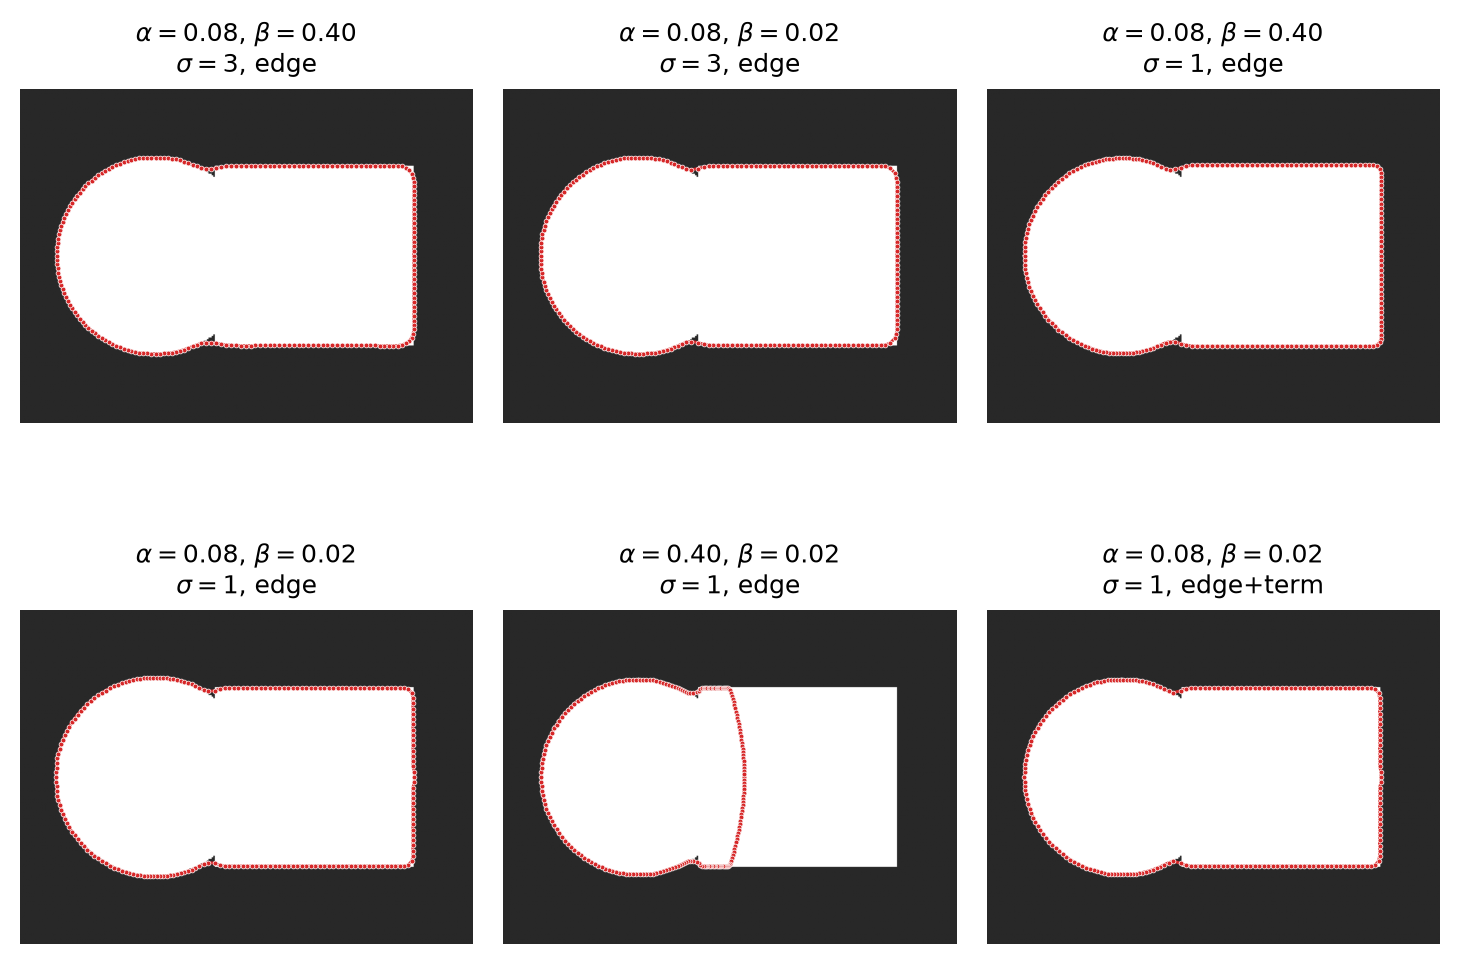
\includegraphics[width=\textwidth]{images/parameters.png}
  \caption{Same initial circle, after it settles. Top left is the default in Figure~\ref{fig:iteration}. Lower $\beta$ sharpens the square's right corners. The notch appears only once $\sigma=1$ and $\beta$ is low. High $\alpha$ leaves the square. Termination smooths the notch.}
  \label{fig:parameters}
\end{figure*}

\subsection{Outside code}

The energies, $A$, and~\eqref{eq:implicit} are from Kass, Witkin, and Terzopoulos \cite{kass1988snakes}.

Blur and Sobel are OpenCV \cite{bradski2000opencv}. The inverse of $A+\gamma I$ is NumPy's dense inverse \cite{harris2020numpy}.

scikit-image's \texttt{active\_contour} was read for that dense inverse and for the $\tanh$ cap \cite{vanderwalt2014scikit}. This implementation uses Kass edge energy, and it does not call scikit-image.

\section{Harder examples}

The same constants as the synthetic run, $\alpha=0.08$, $\beta=0.40$, $\gamma=0.10$, $\kappa=1$, and $\sigma=3$, were used on three photographs. The horseshoe run stopped at step 500. The hand and the quarter were still moving when those runs ended.

\begin{figure*}[t]
  \centering
  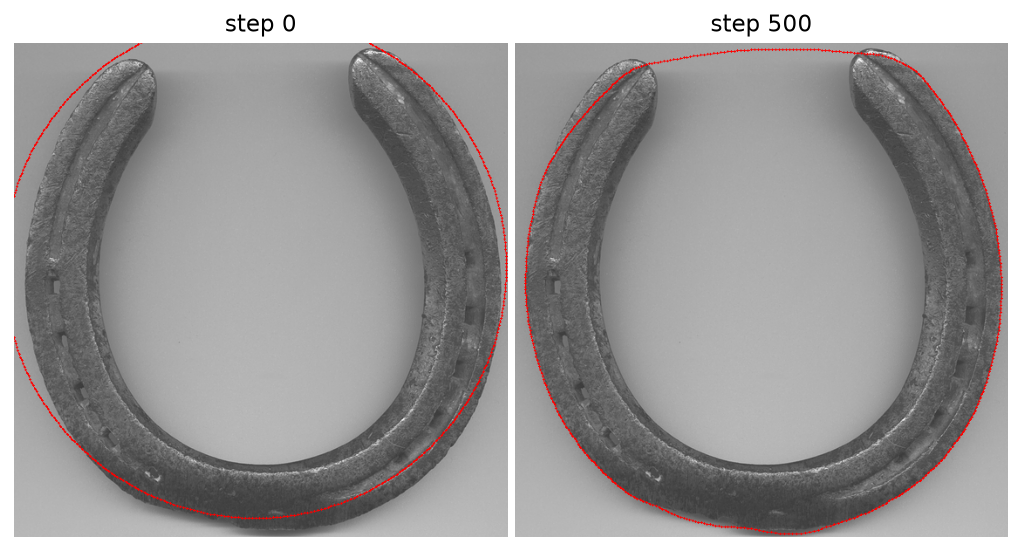
\includegraphics[width=\textwidth]{images/hard_horseshoe.png}
  \caption{Horseshoe. At step 0 the circle sits outside the shoe. At step 500 the beads lie on the outer rim, and a straight segment closes the opening between the two tips.}
  \label{fig:hard-horseshoe}
\end{figure*}

Figure~\ref{fig:hard-horseshoe} starts from a circle around the shoe. By step 500 the loop has tightened onto the outer metal edge. The inner curve stays inside the loop. The two tips are joined by a straight run of beads across empty background.

\begin{figure*}[t]
  \centering
  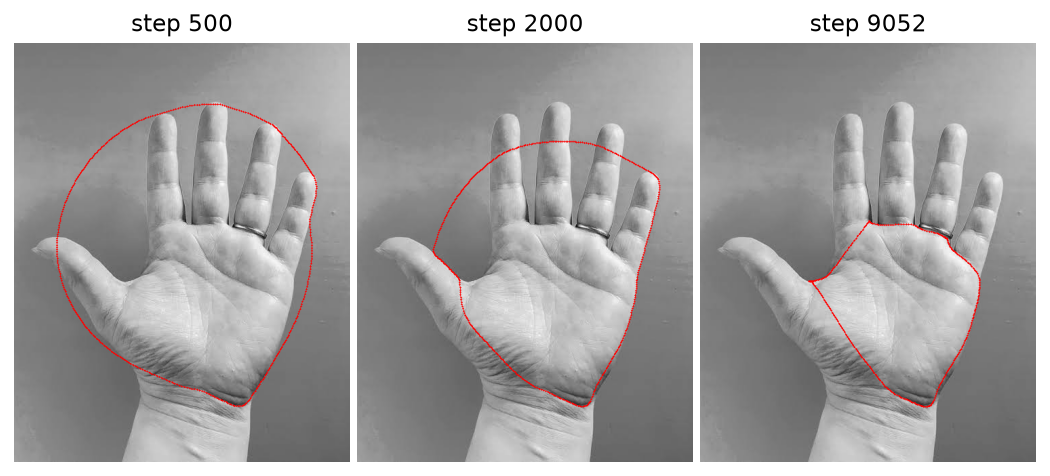
\includegraphics[width=\textwidth]{images/hard_hand.png}
  \caption{Hand. At step 500 the loop touches the fingertips and bridges the gaps. By step 2000 it has left the index and middle fingers. At step 9052 it sits on the palm and the ring.}
  \label{fig:hard-hand}
\end{figure*}

Figure~\ref{fig:hard-hand} starts outside the hand. At step 500 the contour is a smooth oval on the fingertips, the thumb, and the side of the palm. The gaps between the fingers are bridged. By step 2000 the index and middle fingers are outside the loop, and the ring and little finger are still touched at the tips. At step 9052 the loop has left the fingers and lies on the palm, caught on the ring.

\begin{figure*}[t]
  \centering
  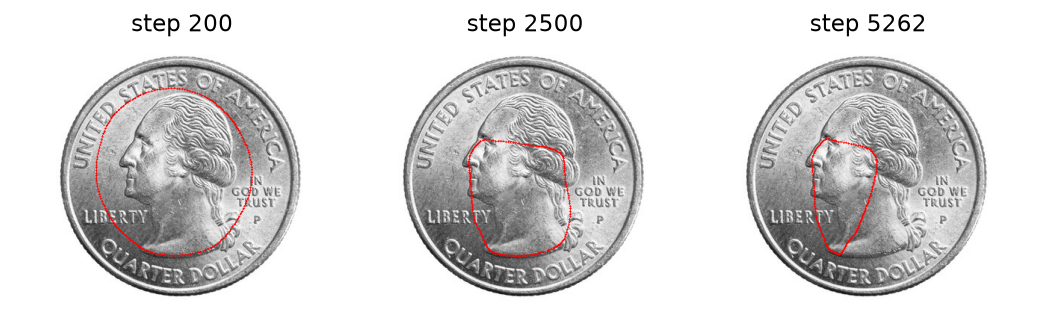
\includegraphics[width=\textwidth]{images/hard_quarter.png}
  \caption{Quarter. At step 200 the beads lie on the profile, the hair, and the neck. By step 2500 the top and the back of the head have been left. At step 5262 the loop is on the face.}
  \label{fig:hard-quarter}
\end{figure*}

Figure~\ref{fig:hard-quarter} starts from a circle around the head, inside the rim of the coin. At step 200 the beads are on the outline: forehead, nose, lips, chin, neck, and the back of the hair. By step 2500 the top of the loop has left the hair and cuts across it, and the back has moved in toward the queue. The nose, mouth, and chin stay on the profile. At step 5262 the contour is a small loop on the face. The hair and the neck are outside it.

\section{Discussion}

On the synthetic blob the interior is empty and the boundary is one edge. The loop tightens onto that edge and stays. These three photographs have more than one place for a bead to sit, and the internal energy keeps shortening and smoothing the loop after it has arrived.

The horseshoe is the notch from Figure~\ref{fig:parameters}, on a larger opening. The outer rim is a strong edge against a flat background, so those beads stay. Across the tips there is no edge. With $\beta=0.40$ the bending term draws the same kind of chord that bridged the disk and the square. A path down the inner curve and back out is longer and more bent, so the straight closing segment is where the loop stops. The run had settled by step 500.

The hand is a set of those openings side by side. At step 500 the beads on the fingertips are on the skin edge, and the beads between the fingers are already off it. Tension pulls along the contour, so a bead on a fingertip is pulled toward the chord in the gap. The loop shortens. Creases in the palm and the ring are edges inside the hand, and the shrinking loop finds them. That is why the contour can touch the outline and later leave it: the neighbors that have already bridged the gap drag the rest off. The run was still moving at step 9052, with the loop on the palm.

The quarter shows the same leaving on a contour that did find the outline. At step 200 the beads are on the profile. The portrait is full of other edges: grooves in the hair, the eye, the mouth, the lettering. The boundary of the hair is a weak edge next to those grooves. A bead that steps inward lands in another well. Because each bead is tied to its neighbors, the beads that are still on the outline are pulled off with it. The nose, lips, and chin are a stronger edge, so that part of the loop stays while the top and the back leave. By step 5262 the short loop on the face is what remains. This is the same shortening that, with $\alpha=0.40$ on the synthetic image, pulled the snake off the square and onto the disk. Here $\alpha$ is still $0.08$; the extra wells inside the head do the pulling.

Figure~\ref{fig:fixing-corners} is the other side of this. A spring on one corner holds that bead out where bending would round it off. These three runs placed no spring and no volcano. Once a bead left the outline, nothing in the update put it back.

\section{Conclusion}

With these constants the snake settles on a short, smooth loop in a strong image well. On the synthetic blob that loop is the object boundary. On the horseshoe it is the outer rim with the opening closed. On the hand it is the palm. On the quarter the beads reach the profile and are then pulled onto the face. A constraint can hold a bead that the image force and the internal energy will not keep there.

\bibliographystyle{plainnat}
\bibliography{refs}

\end{document}
